%\begin{enumerate}[label=\arabic*.,ref=\theenumi]
\begin{enumerate}[label=\thesection.\arabic*.,ref=\thesection.\theenumi]
\numberwithin{equation}{enumi}
%-------------------------------------------------------------------------------------------------%
%2.1.6
\item Find the frequency for which $PM = 90 \degree$.  Assume $H$ to be constant.
\\
%\solution Letting 
%\item Find the frequencies for which phase margins are $90\degree$ and $45\degree$ respectively?\\
\solution $\because \phase{H\brak{f}} = 1$, 
\begin{align}
\phase{G\brak{f_{90}}H\brak{f_{90}}} &= \phase{G\brak{f_{90}}} = 90\degree - 180\degree
\\
&= -90\degree
\label{eq:ee18btech11014_Gpm90}
%\\
%\implies \abs{G\brak{f_{90}}H\brak{f_{90}}} &=1
\end{align}
%
%From \eqref{eq:ee18btech11014_G_ang},
%%
%\begin{multline}
%\phi\brak{f} =
%\\
%-\sbrak{\tan ^{-1}\brak{\frac{f}{10^{5}}}+\tan ^{-1}\brak{\frac{f}{10^{6}}}+\tan ^{-1}\brak{\frac{f}{10^{7}}}}
%\end{multline}
The Bode plot in Fig. 	\ref{fig:ee18btech11014_Bode} shows that 
\begin{align}
\abs{G(f)} < 1, \quad f > 10^8
\end{align}
%
Also, 
\begin{align}
\tan^{-1}\brak{\frac{f}{10^{7}}} \approx 0, \quad f < 10^8
\end{align}

Thus, from  \eqref{eq:ee18btech11014_G_ang} and \eqref{eq:ee18btech11014_Gpm90},
%
\begin{align}
\phi\brak{f} &\approx
-\sbrak{\tan ^{-1}\brak{\frac{f}{10^{5}}}+\tan ^{-1}\brak{\frac{f}{10^{6}}}}
\\
&= -90 \degree
\\
\implies f_{90} &= 3.162 \times 10^{5}
\end{align}
after simplification.
%-------------------------------------------------------------------------------------------------%
\item Find $H$ when the $PM = 90 \degree$.
\\
\solution By definition of the PM, 
\begin{align}
\abs{G\brak{f_{90}}H\brak{f_{90}}} &=1
\\
\implies \abs{H\brak{f_{90}}} &=\frac{1}{\abs{G\brak{f_{90}}}}
\label{eq:ee18btech11014_GH_PM_90}
\end{align}
%
From \eqref{eq:ee18btech11014_G_piece},
\begin{align}
20 \log \abs{G(f)} &= 200 - 20\log(3.162 \times 10^{5})\\
&= 90 dB \\
\implies \abs{G(f)} &= 3.1625 \times 10^{4}
\\
\implies H &= 3.162 \times 10^{-5}
\end{align}
using \eqref{eq:ee18btech11014_GH_PM_90}.
%-------------------------------------------------------------------------------------------------%
\item Design the closed loop circuit for $PM = 90 \degree$
\\
\solution See Fig. 	\ref{fig:ee18btech11014_Closed-Loop Circuit alpha=90}, where Fig. 	\ref{fig:ee18btech11014_Feedback Circuit} is used for the feedback $H$ with $R_M = 0.3162 M \ohm$ and 	$R_F = 10 \ohm$.

\begin{figure}[ht!]
	\begin{center}
		\resizebox{\columnwidth}{!}{\begin{circuitikz}[american]

\draw (2,2)  node[op amp] (OA) {};
\draw (OA.up) -- ++(0, 0.3) node[vcc]{$+10V$};
\draw (OA.down) -- ++(0,-0.3) node[vee]{$-10V$};
\draw (OA.+) -- (0,1.5) to[vsourcesin, l= $v_{s}$] (0,0) node[ground](GND){};
\draw (OA.-) -- (0,2.5) to[R=$10\ohm$] (-2,2.5) node[ground, rotate=270](GND){};
\draw (OA.out) -- (3,2) node[label={below:$v_{a}$}]{};
\draw (3,2) to[R=$10^{2}\ohm$] (5.5,2) node[label={above:$v_{b}$}]{} to[C,l_=$\frac{10^{-9}}{2\pi}F$] (5.5,0) node[ground](GND){};
\draw (5.5,2) to[R=$10^{3}\ohm$] (8,2) node[label={above:$v_{c}$}]{} to[C,l_=$\frac{10^{-9}}{2\pi}F$] (8,0) node[ground](GND){};
\draw (8,2) to[R=$10^{4}\ohm$] (10.5,2) to[C,l_=$\frac{10^{-9}}{2\pi}F$] (10.5,0) node[ground](GND){};
\draw (10.5,2) -- (11.5,2) node[label={above:$v_{o}$}]{};
\draw (10.5,2) -- (10.5,4) to[R=$3.162\times 10^{5}\ohm$] (0,4) -- (0,2.5);

\end{circuitikz}
}
	\end{center}
	\caption{}
	\label{fig:ee18btech11014_Closed-Loop Circuit alpha=90}
\end{figure}
%-------------------------------------------------------------------------------------------------%

\item Using ngspice, find the output of the \ref{fig:ee18btech11014_Closed-Loop Circuit alpha=90} for Unit-Step Signal and Sinusoidal Signal as Input.\\
\solution\\
For Unit-Step Signal as Input,
\begin{align}
T = 24026.91
\end{align}

For Sinusoidal Signal as Input,
\begin{align}
T = 354.5655
\end{align}

Check the following spice file for circuits for the inputs Unit-Step and Sinusoidal Signals respectively.
\begin{lstlisting}
spice/ee18btech11014/ee18btech11014_1.net
spice/ee18btech11014/ee18btech11014_2.net
\end{lstlisting}

Following are the instructions to run the spice file.
\begin{lstlisting}
spice/ee18btech11014/README.md
\end{lstlisting}

Run the following Python Code for Visualising the Responses of the System for both the Inputs.
\begin{lstlisting}
spice/ee18btech11014/EE18BTECH11014_Simulation-1,2.py
\end{lstlisting}

The Responses are shown in Fig.\ref{fig:PM=90}
\begin{figure}[ht!]
	\begin{center}
		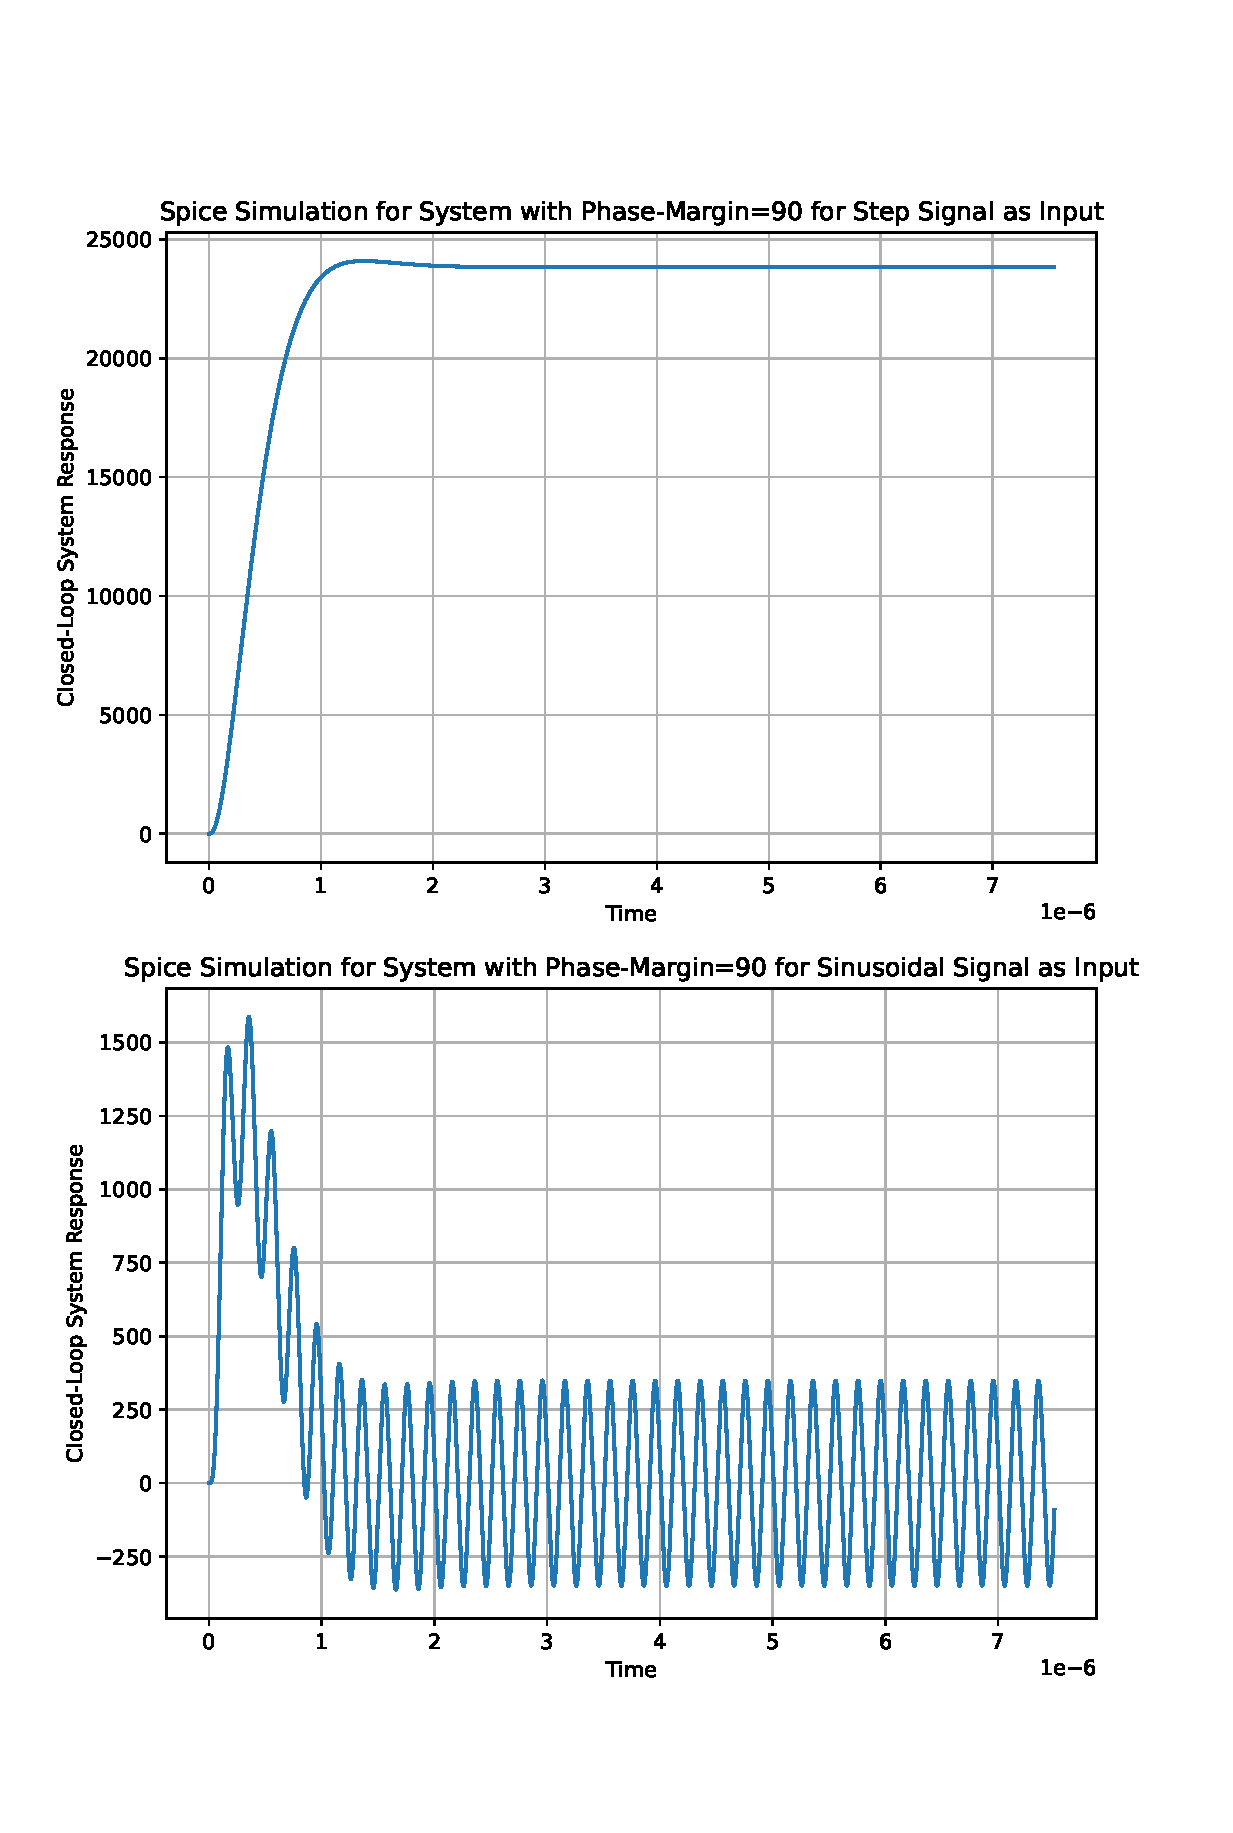
\includegraphics[width=\columnwidth]{./figs/ee18btech11014/ee18btech11014_Spice_Result_PM=90.eps}
	\end{center}
	\caption{}
	\label{fig:PM=90}
\end{figure}


From Simulation, for Unit-Step Signal as Input,
\begin{align}
T = 23842.97
\end{align}

From Simulation, for Sinusoidal Signal as Input,
\begin{align}
T = 349.01
\end{align}

Percentage of Error from Theoritical and Simulation results when Unit-Step Signal is given as Input is $0.77\%$.

Percentage of Error from Theoritical and Simulation results when Sinusoidal Signal is given as Input is $1.59\%$.
%-------------------------------------------------------------------------------------------------%
\item Repeat all the above for $PM = 45\degree$.
%-------------------------------------------------------------------------------------------------%

%-\tan^{-1}\left(f/10^{5}\right)-\tan^{-1}\left(f/10^{6}\right) = -90\\
%\tan^{-1}\left(f/10^{5}\right)+\tan^{-1}\left(f/10^{6}\right) = 90\\
%\tan^{-1}\left(f/10^{5}\right) = 90-\tan^{-1}\left(f/10^{6}\right)\\
%\tan^{-1}\left(f/10^{5}\right) = \cot^{-1}\left(f/10^{6}\right)\\
%\tan^{-1}\left(f/10^{5}\right) = \tan^{-1}\left(10^{6}/f\right)\\
%f^{2} = 10^{11}\\
%f = 3.162 \times 10^{5}
%\end{align}
%
%So, the approximate value of $f$ at which Phase Margin is $90\degree$ is $f=3.162 \times 10^{5} Hz$.\\

%Similarly let Phase Margin be $\alpha = 45\degree$. Then,
%\begin{align}
%\alpha = \phi - (-180\degree)\\
%\phi = -180\degree + \alpha\\
%\phi = -135\degree
%\end{align}
%
%So, by the definition of Phase-Margin, at $\phi = -135\degree$ , $|GH| = 1 $.  The value of $\phi = -135\degree$ aproximately at poles $f=10^{6} Hz$. 
%
%So, the approximate value of $f$ at which Phase Margin is $45\degree$ is $f=10^{6}$.\\
%%-------------------------------------------------------------------------------------------------%
%%2.1.7
%\item Find the minimum values of Closed-Loop Voltage Gain for which phase margins are $90\degree$ and  $45\degree$ respectively\\
%\solution\\
%For $\alpha=90\degree$,
%\begin{align}
%f=3.162 \times 10^{5}
%\end{align}
%By substituting $f$ in Open-Loop Gain $G(f)$ (assuming poles are far part), 
%\begin{align}
%G(f) = 200 - 20log(3.162 \times 10^{5})\\
%G(f) = 90 dB \\
%G = 3.1625 \times 10^{4}
%\end{align}
%
%At that $f=3.162 \times 10^{5}$, 
%\begin{align}
%H = \frac{1}{G}\\
%H = 3.162 \times 10^{-5}
%\end{align}
%
%The minimum value of Closed-Loop Gain occurs at $|GH| \gg 1$ and the value of Closed-Loop Gain is $T=\frac{1}{H}$
%
%\begin{align}
%T = \frac{1}{H} = 3.1625 \times 10^{4}
%\end{align}
%
%\textbf{So, The minimum value of Closed-Loop Gain with Phase Margin equal to $\alpha=90\degree$ is $T_{min} = 3.1625 \times 10^{4}$.}\\
%
%For $\alpha=45\degree$,
%\begin{align}
%f=10^{6}
%\end{align}
%By substituting $f$ in Open-Loop Gain $G(f)$ (assuming poles are far part), 
%\begin{align}
%G(f) = 200 - 20log(10^{6})\\
%G(f) = 80 dB \\
%G = 10^{4}
%\end{align}
%
%At that $f = 10^{6}$, 
%\begin{align}
%H = \frac{1}{G}\\
%H = 10^{-4}
%\end{align}
%
%The minimum value of Closed-Loop Gain occurs at $|GH| \gg 1$ and the value of Closed-Loop Gain is $T=\frac{1}{H}$
%
%\begin{align}
%T = \frac{1}{H} = 10^{4}
%\end{align}
%
%\textbf{So, The minimum value of Closed-Loop Gain with Phase Margin equal to $\alpha=45\degree$ is $T_{min} = 10^{4}$.}\\
%%-------------------------------------------------------------------------------------------------%
%
%\item Design a Feedback circuit for Phase Margin $\alpha=45^{\circ}$.\\
%\solution
%\begin{figure}[ht!]
%	\begin{center}
%		\resizebox{\columnwidth/2}{!}{\begin{circuitikz}[american]
\ctikzset{tripoles/mos style/arrows}
\draw (1,2) to[short, -o] (0,2) node[label={below:$v_{o}$}]{};
\draw (1,2) to[R=$100k\ohm$] (2,2) -- (3,2) to[R=$10\ohm$] (3,0) node[ground](GND){};
\draw (3,2) to[short, -o] (4,2) node[label={below:$v_{f}$}]{};
\end{circuitikz}
}
%	\end{center},
%	\caption{}
%	\label{fig:ee18btech11014_alpha=45}
%\end{figure}
%\begin{align}
%v_{f} = \frac{10}{10 + 10^{5}} \times v_{o}\\
%v_{f} \approx 10^{-4} v_{o}\\
%\frac{v_{f}}{v_{o}} \approx 10^{-4}\\
%H(s) = 10^{-4}
%\end{align}
%%-------------------------------------------------------------------------------------------------%
%
%\item Design a Feedback circuit for Phase Margin $\alpha=90^{\circ}$.\\
%\solution
%\begin{figure}[ht!]
%	\begin{center}
%		\resizebox{\columnwidth/2}{!}{\begin{circuitikz}[american]
\ctikzset{tripoles/mos style/arrows}
\draw (1,2) to[short, -o] (0,2) node[label={below:$v_{o}$}]{};
\draw (1,2) to[R=$0.3162 M\ohm$] (2,2) -- (3,2) to[R=$10\ohm$] (3,0) node[ground](GND){};
\draw (3,2) to[short, -o] (4,2) node[label={below:$v_{f}$}]{};
\end{circuitikz}
}
%	\end{center},
%	\caption{}
%	\label{fig:ee18btech11014_alpha=90}
%\end{figure}
%\begin{align}
%v_{f} = \frac{10}{10 + 3.162\times 10^{5}} \times v_{o}\\
%v_{f} \approx 3.162\times 10^{-5} v_{o}\\
%\frac{v_{f}}{v_{o}} \approx 3.162\times 10^{-5}\\
%H(s) = 3.162\times 10^{-5}
%\end{align}
%%-------------------------------------------------------------------------------------------------%
%
%\item  Design a Closed-Loop Transfer Function by combining both the Open-Loop and Feedback Circuits for phase Margin $\alpha=45^{\circ}$. Also draw its Equivalent Circuit\\
%\solution\\
%The Closed-Loop Circuit is
%\begin{figure}[ht!]
%	\begin{center}
%		\resizebox{\columnwidth}{!}{\begin{circuitikz}[american]

\draw (2,2)  node[op amp] (OA) {};
\draw (OA.up) -- ++(0, 0.3) node[vcc]{$+10V$};
\draw (OA.down) -- ++(0,-0.3) node[vee]{$-10V$};
\draw (OA.+) -- (0,1.5) to[vsourcesin, l= $v_{s}$] (0,0) node[ground](GND){};
\draw (OA.-) -- (0,2.5) to[R=$10\ohm$] (-2,2.5) node[ground, rotate=270](GND){};
\draw (OA.out) -- (3,2) node[label={below:$v_{a}$}]{};
\draw (3,2) to[R=$10^{2}\ohm$] (5.5,2) node[label={above:$v_{b}$}]{} to[C,l_=$\frac{10^{-9}}{2\pi}F$] (5.5,0) node[ground](GND){};
\draw (5.5,2) to[R=$10^{3}\ohm$] (8,2) node[label={above:$v_{c}$}]{} to[C,l_=$\frac{10^{-9}}{2\pi}F$] (8,0) node[ground](GND){};
\draw (8,2) to[R=$10^{4}\ohm$] (10.5,2) to[C,l_=$\frac{10^{-9}}{2\pi}F$] (10.5,0) node[ground](GND){};
\draw (10.5,2) -- (11.5,2) node[label={above:$v_{o}$}]{};
\draw (10.5,2) -- (10.5,4) to[R=$10^{5}\ohm$] (0,4) -- (0,2.5);

\end{circuitikz}
}
%	\end{center}
%	\caption{}
%	\label{fig:ee18btech11014_Closed-Loop Circuit alpha=45}
%\end{figure}
%
%The Equivalent Circuit of Closed-Loop Circuit is
%\begin{figure}[ht!]
%	\begin{center}
%		\resizebox{\columnwidth}{!}{\begin{circuitikz}[american]-1
\draw (-3,0) node[ground](GND){} to[vsourcesin, l= $v_{s}$] (-3,2) to[short,-o] (0.25,2) node[label={below:$+$}]{};
\draw (0,0.1) to[R=$10\ohm$,v=$v_{f}$] (-2,0.1) node[ground](GND){}; 
\draw (0,0.1) -- (1,0.1) -- (1,4) to[R=$10^{5}\ohm$] (10.5,4) -- (10.5,2);


\draw (0.25,0.1) to[short,-o] (0.25,0.1) node[label={above:$-$}]{};
\draw (0.25,0.625) node[label={$v_{i}$}] {};


\draw (3,2) node[label={above:$v_{a}$}]{};
\draw (3,0) node[ground](GND){} to[vsourcesin, l= $10^5 v_{i}$] (3,2);
\draw (3,2) to[R=$10^{2}\ohm$] (5.5,2) node[label={above:$v_{b}$}]{} to[C,l_=$\frac{10^{-9}}{2\pi}F$] (5.5,0) node[ground](GND){};
\draw (5.5,2) to[R=$10^{3}\ohm$] (8,2) node[label={above:$v_{c}$}]{} to[C,l_=$\frac{10^{-9}}{2\pi}F$] (8,0) node[ground](GND){};
\draw (8,2) to[R=$10^{4}\ohm$] (10.5,2) to[C,l_=$\frac{10^{-9}}{2\pi}F$] (10.5,0) node[ground](GND){};
\draw (10.5,2) -- (11.5,2) node[label={above:$v_{o}$}]{};

\end{circuitikz}
}
%	\end{center},
%	\caption{}
%	\label{fig:ee18btech11014_Closed-Loop Equivalent Circuit alpha=45}
%\end{figure}
%
%From the Equivalent Circuit Diagram,
%\begin{align}
%G(s) = \dfrac{10^5}{\left(1+\frac{s}{2\pi 10^{5}}\right)\left(1+\frac{s}{2\pi 10^{6}}\right)\left(1+\frac{s}{2\pi 10^{7}}\right)}\\
%H(s) = \frac{v_{f}}{v_{o}} = 10^{-4}
%\end{align}
%
%The Closed-Loop Gain,
%\begin{align}
%v_{i} = v_{s} - v_{f}\\
%\frac{v_{o}}{G} = v_{s} - Hv_{o}\\
%\frac{v_{o}}{v_{s}} = \frac{G}{1+GH}
%\end{align}
%
%So, the Closed-Loop Gain,
%\begin{align}
%T(s) = \frac{v_{o}}{v_{s}} = \dfrac{10^5}{10 + \left(1+s\frac{s}{2\pi 10^{5}}\right)\left(1+\frac{s}{2\pi 10^{6}}\right)\left(1+j\frac{s}{2\pi 10^{7}}\right)}
%\end{align}
%%-------------------------------------------------------------------------------------------------%
%
%\item  Design a Closed-Loop Transfer Function by combining both the Open-Loop and Feedback Circuits for phase Margin $\alpha=90^{\circ}$. Also draw its Equivalent Circuit\\
%\solution\\
%The Closed-Loop Circuit is
%\begin{figure}[ht!]
%	\begin{center}
%		\resizebox{\columnwidth}{!}{\begin{circuitikz}[american]

\draw (2,2)  node[op amp] (OA) {};
\draw (OA.up) -- ++(0, 0.3) node[vcc]{$+10V$};
\draw (OA.down) -- ++(0,-0.3) node[vee]{$-10V$};
\draw (OA.+) -- (0,1.5) to[vsourcesin, l= $v_{s}$] (0,0) node[ground](GND){};
\draw (OA.-) -- (0,2.5) to[R=$10\ohm$] (-2,2.5) node[ground, rotate=270](GND){};
\draw (OA.out) -- (3,2) node[label={below:$v_{a}$}]{};
\draw (3,2) to[R=$10^{2}\ohm$] (5.5,2) node[label={above:$v_{b}$}]{} to[C,l_=$\frac{10^{-9}}{2\pi}F$] (5.5,0) node[ground](GND){};
\draw (5.5,2) to[R=$10^{3}\ohm$] (8,2) node[label={above:$v_{c}$}]{} to[C,l_=$\frac{10^{-9}}{2\pi}F$] (8,0) node[ground](GND){};
\draw (8,2) to[R=$10^{4}\ohm$] (10.5,2) to[C,l_=$\frac{10^{-9}}{2\pi}F$] (10.5,0) node[ground](GND){};
\draw (10.5,2) -- (11.5,2) node[label={above:$v_{o}$}]{};
\draw (10.5,2) -- (10.5,4) to[R=$3.162\times 10^{5}\ohm$] (0,4) -- (0,2.5);

\end{circuitikz}
}
%	\end{center}
%	\caption{}
%	\label{fig:ee18btech11014_Closed-Loop Circuit alpha=90}
%\end{figure}
%
%The Equivalent Circuit of Closed-Loop Circuit is
%\begin{figure}[ht!]
%	\begin{center}
%		\resizebox{\columnwidth}{!}{\begin{circuitikz}[american]-1
\draw (-3,0) node[ground](GND){} to[vsourcesin, l= $v_{s}$] (-3,2) to[short,-o] (0.25,2) node[label={below:$+$}]{};
\draw (0,0.1) to[R=$10\ohm$,v=$v_{f}$] (-2,0.1) node[ground](GND){}; 
\draw (0,0.1) -- (1,0.1) -- (1,4) to[R=$3.162\times 10^{5}\ohm$] (10.5,4) -- (10.5,2);


\draw (0.25,0.1) to[short,-o] (0.25,0.1) node[label={above:$-$}]{};
\draw (0.25,0.625) node[label={$v_{i}$}] {};


\draw (3,2) node[label={above:$v_{a}$}]{};
\draw (3,0) node[ground](GND){} to[vsourcesin, l= $10^5 v_{i}$] (3,2);
\draw (3,2) to[R=$10^{2}\ohm$] (5.5,2) node[label={above:$v_{b}$}]{} to[C,l_=$\frac{10^{-9}}{2\pi}F$] (5.5,0) node[ground](GND){};
\draw (5.5,2) to[R=$10^{3}\ohm$] (8,2) node[label={above:$v_{c}$}]{} to[C,l_=$\frac{10^{-9}}{2\pi}F$] (8,0) node[ground](GND){};
\draw (8,2) to[R=$10^{4}\ohm$] (10.5,2) to[C,l_=$\frac{10^{-9}}{2\pi}F$] (10.5,0) node[ground](GND){};
\draw (10.5,2) -- (11.5,2) node[label={above:$v_{o}$}]{};

\end{circuitikz}
}
%	\end{center},
%	\caption{}
%	\label{fig:ee18btech11014_Closed-Loop Equivalent Circuit alpha=90}
%\end{figure}
%
%From the Equivalent Circuit Diagram,
%\begin{align}
%G(s) = \dfrac{10^5}{\left(1+\frac{s}{2\pi 10^{5}}\right)\left(1+\frac{s}{2\pi 10^{6}}\right)\left(1+\frac{s}{2\pi 10^{7}}\right)}\\
%H(s) = \frac{v_{f}}{v_{o}} = 3.162\times 10^{-5}
%\end{align}
%
%The Closed-Loop Gain,
%\begin{align}
%v_{i} = v_{s} - v_{f}\\
%\frac{v_{o}}{G} = v_{s} - Hv_{o}\\
%\frac{v_{o}}{v_{s}} = \frac{G}{1+GH}
%\end{align}
%
%So, the Closed-Loop Gain,
%\begin{align}
%T(s) = \frac{v_{o}}{v_{s}} = \dfrac{10^5}{3.162 + \left(1+s\frac{s}{2\pi 10^{5}}\right)\left(1+\frac{s}{2\pi 10^{6}}\right)\left(1+j\frac{s}{2\pi 10^{7}}\right)}
%\end{align}
\end{enumerate}
